% The shape each hypothesis implies; compile with pdflatex. Sketches, drawn to no estimate.
\documentclass[border=4pt]{standalone}
\usepackage[T1]{fontenc}
\usepackage{helvet,amsmath,tikz}
\renewcommand{\familydefault}{\sfdefault}
\definecolor{calm}{RGB}{0,114,178}
\definecolor{stress}{RGB}{213,94,0}
\newcommand{\sketchaxes}{%
  \draw[->,thin] (0,0)--(3.1,0);
  \node[font=\scriptsize] at (1.55,-0.55) {debt to GDP};
  \draw[->,thin] (0,0)--(0,2.5) node[midway,above,rotate=90,font=\scriptsize]{depreciation};}
\begin{document}
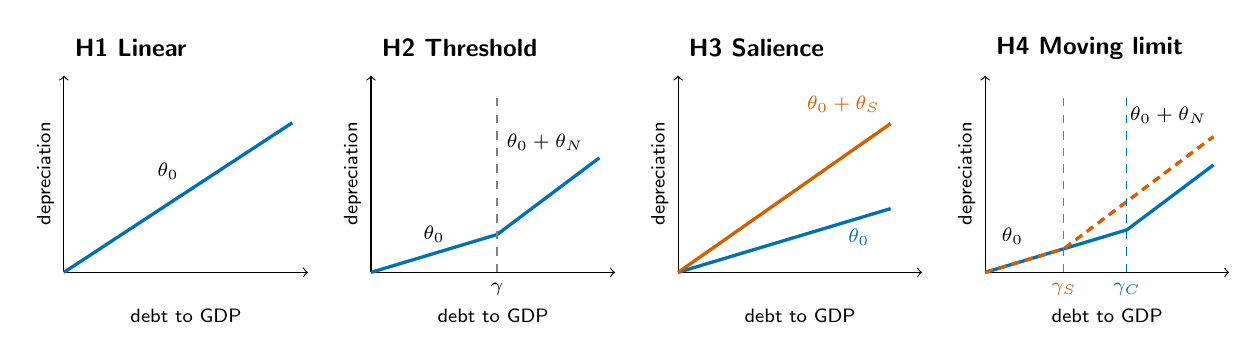
\begin{tikzpicture}[line width=1.2pt]
  \begin{scope}
    \sketchaxes
    \draw[calm] (0,0)--(2.9,1.9) node[pos=0.55,above left,font=\scriptsize,black]{$\theta_0$};
    \node[font=\small\bfseries,anchor=west] at (0,2.85) {H1 Linear};
  \end{scope}
  \begin{scope}[xshift=3.9cm]
    \sketchaxes
    \draw[calm] (0,0)--(1.6,0.48) node[pos=0.5,above,font=\scriptsize,black]{$\theta_0$};
    \draw[calm] (1.6,0.48)--(2.9,1.455) node[pos=0.95,above left,font=\scriptsize,black]{$\theta_0+\theta_N$};
    \draw[dashed,thin,gray] (1.6,0)--(1.6,2.3);
    \node[font=\scriptsize,below] at (1.6,0) {$\gamma$};
    \node[font=\small\bfseries,anchor=west] at (0,2.85) {H2 Threshold};
  \end{scope}
  \begin{scope}[xshift=7.8cm]
    \sketchaxes
    \draw[calm] (0,0)--(2.7,0.81) node[pos=0.85,below,font=\scriptsize,calm]{$\theta_0$};
    \draw[stress] (0,0)--(2.7,1.89) node[pos=1,above left,font=\scriptsize,stress]{$\theta_0+\theta_S$};
    \node[font=\small\bfseries,anchor=west] at (0,2.85) {H3 Salience};
  \end{scope}
  \begin{scope}[xshift=11.7cm]
    \sketchaxes
    \draw[calm] (0,0)--(1.8,0.54)--(2.9,1.365);
    \draw[stress,dash pattern=on 3pt off 2pt] (0,0)--(1.0,0.30)--(2.9,1.725);
    \draw[dashed,thin,stress] (1.0,0)--(1.0,2.3);
    \draw[dashed,thin,calm] (1.8,0)--(1.8,2.3);
    \node[font=\scriptsize,below,stress] at (1.0,0) {$\gamma_S$};
    \node[font=\scriptsize,below,calm] at (1.8,0) {$\gamma_C$};
    \node[font=\scriptsize,anchor=south east] at (0.62,0.22) {$\theta_0$};
    \node[font=\scriptsize,anchor=south east] at (2.95,1.75) {$\theta_0+\theta_N$};
    \node[font=\small\bfseries,anchor=west] at (0,2.85) {H4 Moving limit};
  \end{scope}
\end{tikzpicture}
\end{document}
